% =====================================================================
% Práctica 1 · Robótica Inteligente Aplicada · Memoria
% pdfLaTeX (Overleaf): usa Carlito, métricamente igual que Calibri.
% XeLaTeX/LuaLaTeX con Calibri instalada: usa Calibri.
% Las figuras se buscan en ../figuras/ y en figuras/.
% =====================================================================
\documentclass[11pt,a4paper]{article}

\usepackage{iftex}
\ifPDFTeX
  \usepackage[T1]{fontenc}
  \usepackage[utf8]{inputenc}
  \usepackage[sfdefault,lining]{carlito}
\else
  \usepackage{fontspec}
  \IfFontExistsTF{Calibri}{\setmainfont{Calibri}}{\setmainfont{Carlito}}
\fi
\usepackage[spanish,es-noshorthands,es-tabla]{babel}
\usepackage[a4paper,margin=2cm]{geometry}
\usepackage{amsmath}
\usepackage{icomma}
\usepackage{graphicx}
\usepackage{booktabs,tabularx}
\usepackage[font=small,labelfont=bf,skip=3pt]{caption}
\usepackage{enumitem}
\usepackage{titlesec}
\usepackage[hidelinks]{hyperref}

\graphicspath{{../figuras/}{figuras/}}
\setlength{\parindent}{0pt}
\setlength{\parskip}{4pt}
\setlist{nosep,leftmargin=12pt}
\titleformat{\section}{\large\bfseries}{\thesection.}{0.4em}{}
\titleformat{\subsection}{\normalsize\bfseries}{\thesubsection.}{0.4em}{}
\titlespacing*{\section}{0pt}{8pt}{3pt}
\titlespacing*{\subsection}{0pt}{5pt}{2pt}
\newcolumntype{Y}{>{\raggedright\arraybackslash}X}
\newcommand{\cod}[1]{\texttt{\small #1}}

\begin{document}

{\Large\bfseries Práctica 1 · Seguimiento de un vehículo en la ciudad\par}
\vspace{2pt}
{\small Robótica Inteligente Aplicada · Grado en Inteligencia Artificial · Universidade da Coruña · Curso 2026/27\\
[Nombre y apellidos 1] · [Nombre y apellidos 2]\par}

\section{Introducción}

Se entrena por refuerzo un controlador continuo para que un Robobo (el \emph{seguidor}) circule detrás del
vehículo guía de \emph{Follow City} en RoboboSim, que lleva una pelota verde. El seguidor debe mantener la
separación con la pelota entre 0,20 y 0,45~m sin chocar ($<0{,}12$~m), sin perder al guía ($>0{,}90$~m o
más de 3~s sin verlo) y sin salirse de la carretera, sólo con sus sensores y a través de ROS~2. Se estudian
tres configuraciones del guía: \textbf{C1} (crucero 10--10), \textbf{C2} (crucero 10--40) y \textbf{C3}
(variable 10--40). En cada una se prueban SAC y PPO (Stable-Baselines3), se compara con una política
aleatoria y se evalúa con el protocolo del anexo~B del enunciado: episodios de 120~s, política determinista y
reinicio de la escena.

\section{Archivos y manual de ejecución}

\begin{table}[h]
\centering\small
\caption{Archivos entregados.}
\label{tab:archivos}
\begin{tabularx}{\linewidth}{@{}lY@{}}
\toprule
Archivo & Contenido \\
\midrule
\cod{p1\_seguidor\_env.py} & Entorno de Gymnasium: observación, acción, paso sincronizado, terminación y reinicio. \\
\cod{p1\_recompensa.py} & Función de recompensa. \\
\cod{p1\_seguidor.py} & Programa principal: calibración, línea base, entrenamiento, evaluación y ejecución. \\
\cod{p1\_simulador.py} & Conexión directa con RoboboSim (verdad del terreno, reinicio y colocación del seguidor). \\
\cod{p1\_protocolo.py} & Evaluador del anexo~B: métricas a partir de los CSV por paso. \\
\cod{p1\_curvas.py}, \cod{p1\_figuras.py} & Curvas de aprendizaje y figuras de caracterización. \\
\cod{p1\_config.json} & Parámetros de calibración, escenario y protocolo, cada uno justificado. \\
\cod{p1\_logs/definitivos/} & Por entrenamiento: \cod{modelo.zip}, \cod{config.json} y \cod{monitor.csv} (un episodio por fila). \\
\cod{p1\_eval/definitivos/} & Registro por paso de cada episodio de evaluación (CSV). \\
\bottomrule
\end{tabularx}
\end{table}

\textbf{Puesta en marcha.} RoboboSim abierto en \emph{Follow City}, con el guía configurado (C1: Mode~1, 10--10;
C2: Mode~1, 10--40; C3: Mode~2, 10--40) y la ventana en primer plano, porque sin foco RoboboSim congela la
física. Dentro del contenedor, en un terminal se lanza el puente sólo con el módulo de blobs:
\begin{quote}\small\ttfamily
ros2 run robobo\_ros2 robobo\_container --ros-args -p ip:=host.docker.internal -p modules:="['blob']"
\end{quote}
y en otro, desde \cod{/docker-ros/ws}, se ejecuta \cod{p1\_seguidor.py} en este orden:
\begin{enumerate}
\item \textbf{Calibración} (una vez; guarda en \cod{p1\_config.json}): \cod{--calibrar-movimiento},
\cod{--barrido-tilt --guardar}, \cod{--caracterizar --guardar}, \cod{--grabar-linea} y, por último,
\cod{--comprobar}.
\item \textbf{Línea base:} \cod{--aleatorio --episodios 10 --etiqueta C1}.
\item \textbf{Entrenamiento:} \cod{--entrenar --algoritmo sac --pasos 20000 --semilla 0 --etiqueta C1}. Para
cuando cumple el criterio de éxito o se estanca; \cod{--sin-parada} fija el número de pasos y
\cod{--continuar <modelo.zip>} reanuda.
\item \textbf{Evaluación:} \cod{--evaluar --modelo p1\_logs/definitivos/sac\_C1\_s0/modelo --configuracion C1
--episodios 3} (también \cod{--modelo aleatoria}).
\item \textbf{Resultados:} \cod{python3 p1\_protocolo.py "p1\_eval/definitivos/*.csv"} (tablas) y
\cod{python3 p1\_curvas.py --grupo "SAC=p1\_logs/definitivos/sac\_C1\_s[0-9]" ...} (curvas).
\end{enumerate}

\section{Diseño común del entorno}

\textbf{Caracterización.} Medida con herramientas propias (Figuras~\ref{fig:caract} y~\ref{fig:tilt}): el
detector da $\approx$1,8 imágenes nuevas por segundo; con la cámara a 100° la pelota se ve de 0,2 a 1,2~m; la
distancia se estima con $d=2{,}616\cdot\text{size}^{-0{,}384}$ (error 0,09~m) y el campo de visión es de 46,6°.
El robot va 1,975 veces (lineal) y 1,722 veces (angular) más rápido de lo que pide \cod{cmd\_vel}.

\textbf{Observación} (11 componentes, sólo de sensores del seguidor): pelota visible; $x$ e $y$ del blob;
distancia estimada; velocidad de la pelota en la imagen; velocidad de alejamiento; velocidad estimada del guía
($v_{\text{propia}}+\dot{\hat d}$, que permite detectar sus cambios de velocidad); tiempo sin ver la pelota;
infrarrojo frontal; y la acción anterior. Todo normalizado con magnitudes físicas.

\textbf{Acción} continua, publicada en \cod{cmd\_vel}: $v\in[0;\,0{,}35]$~m/s (1,6 veces la velocidad del guía) y
$w\in[-0{,}6;\,0{,}6]$~rad/s, acotada para que un paso no saque de la imagen una pelota centrada. C2 se entrenó
con $v_{\min}=-0{,}05$; al ver que PPO retrocedía con frecuencia se fijó $v_{\min}=0$ para C1 y C3.

\textbf{Recompensa}, sin pesos ajustados a mano:
$r = C_{\text{sep}}(d)\cdot C_{\text{ori}}(\theta) + [\gamma\Phi(d')-\Phi(d)] - 1_{\text{fallo}}$, con
$\gamma=0{,}99$. $C_{\text{sep}}$ vale 1 en la banda y baja linealmente a 0 en 0,12 y 0,90~m; $C_{\text{ori}}$
vale 1 con la pelota a menos de 15° del centro y 0 en el borde de la imagen o si no se ve. $\Phi$ es un
moldeado basado en potencial (máximo en 0,325~m), que no cambia la política óptima y enseña a acelerar o frenar
con el guía. El producto obliga a cumplir los dos objetivos a la vez sin decidir cuánto vale cada uno.

\textbf{Paso y reinicio.} Cada \cod{step()} mantiene la orden 0,2~s y espera una imagen nueva del detector, así
que la observación siempre es posterior a la acción ($\approx$0,56--0,64~s por paso). Los episodios terminan por
los fallos del protocolo o por salir de la calzada, y se truncan a los 300 pasos. Al reiniciar, un 30~\% de las
veces se reinicia la escena (como en la evaluación) y un 70~\% se coloca al seguidor detrás de la pelota con el
guía en marcha.

\textbf{Entrenamiento.} Los primeros 1000 pasos de SAC son de avance hacia la pelota (calentamiento) en lugar de
acciones al azar. La parada temprana corta por éxito (80~\% de los últimos 20 episodios completos) o por
estancamiento (sin mejorar un 5~\% en 3000 pasos). Hiperparámetros por defecto de SB3, salvo
\cod{learning\_starts}~=~1000 (SAC) y \cod{n\_steps}~=~512 (PPO).

\section{Resultados por configuración}

\subsection{C1: crucero 10--10}
SAC se entrenó con tres semillas hasta el criterio de parada; PPO, con una. Curvas en las
Figuras~\ref{fig:C1} y~\ref{fig:C1mod}.

\begin{table}[h]
\centering\small
\caption{C1. Entrenamiento (últimos 20 episodios) y evaluación con el protocolo (3 episodios de 120~s).}
\label{tab:C1}
\setlength{\tabcolsep}{3.5pt}
\begin{tabular}{@{}lrcrccccc@{}}
\toprule
& \multicolumn{3}{c}{Entrenamiento} & \multicolumn{5}{c}{Evaluación} \\
\cmidrule(lr){2-4}\cmidrule(l){5-9}
Política & Pasos & Parada & Compl. & Compl. & En banda & Sep. media & $|$Desv.$|$ & En carril \\
\midrule
Aleatoria & --- & --- & 0~\% & 0/3 & 40,0~\% & 0,195~m & 16,0° & 100~\% \\
PPO s0 & 6\,624 & --- & 0~\% & \multicolumn{5}{c}{no evaluado} \\
\textbf{SAC s0} & 9\,431 & éxito & 80~\% & \textbf{3/3} & \textbf{100~\%} & 0,314~m & \textbf{2,1°} & 100~\% \\
SAC s1 & 7\,817 & éxito & 80~\% & 3/3 & 100~\% & 0,311~m & 2,6° & 100~\% \\
SAC s2 & 10\,264 & estancamiento & 50~\% & 2/3 & 100~\% & 0,307~m & 3,8° & 99,3~\% \\
\bottomrule
\end{tabular}
\end{table}

Las tres semillas de SAC aprenden casi igual: superan a la aleatoria hacia el paso 2000 y al final el 80~\% de
los episodios se completan. Al principio casi todos los episodios acaban en colisión, porque el guía va muy
despacio y el calentamiento avanza deprisa; después la causa dominante pasa a ser «sin pelota» y finalmente el
tiempo. En evaluación SAC completa 8 de 9 episodios y pasa el 100~\% del tiempo en banda. PPO no se separa de la
aleatoria en todo el entrenamiento (episodios de $\approx$9 pasos).

\textbf{Política elegida: SAC s0.} Completa los 3 episodios, siempre en banda, con la menor desviación media
(2,1°); s1 es prácticamente equivalente y aprendió antes.

\subsection{C2: crucero 10--40}
SAC s0 cumplió el criterio de éxito a los 12\,648 pasos, que se usaron como presupuesto fijo para PPO y para SAC
s1 y s2. Después se extendieron SAC s2 (hasta el criterio de éxito) y PPO (más del doble de pasos). Curvas en
las Figuras~\ref{fig:C2}--\ref{fig:C2ext}.

\begin{table}[h]
\centering\small
\caption{C2. Entrenamiento (últimos 20 episodios) y evaluación con el protocolo (3 episodios de 120~s).}
\label{tab:C2}
\setlength{\tabcolsep}{3.5pt}
\begin{tabular}{@{}lrrccccc@{}}
\toprule
& \multicolumn{2}{c}{Entrenamiento} & \multicolumn{5}{c}{Evaluación} \\
\cmidrule(lr){2-3}\cmidrule(l){4-8}
Política & Pasos & Compl. & Compl. & En banda & Sep. media & $|$Desv.$|$ & En carril \\
\midrule
Aleatoria & --- & 0~\% & 0/3 & 17,1~\% & 0,619~m & 22,5° & 82,9~\% \\
PPO s0 & 13\,067 & 0~\% & 1/3 & 38,7~\% & 0,494~m & 11,7° & 94,3~\% \\
SAC s0 & 12\,648 & 80~\% & 2/3 & 97,9~\% & 0,323~m & 6,4° & 100~\% \\
\textbf{SAC s1} & 12\,550 & 75~\% & \textbf{3/3} & \textbf{98,2~\%} & 0,338~m & \textbf{4,6°} & 100~\% \\
SAC s2 & 12\,524 & 25~\% & 1/3 & 96,9~\% & 0,342~m & 6,9° & 98,9~\% \\
\midrule
SAC s2 extendido & 17\,616 & 80~\% & 3/3 & 96,7~\% & 0,341~m & 5,5° & 100~\% \\
PPO extendido & 28\,421 & 0~\% & 2/3 & 63,9~\% & 0,415~m & 8,7° & 92,1~\% \\
\bottomrule
\end{tabular}
\end{table}

Con el mismo presupuesto, SAC está el 97,7~$\pm$~0,7~\% del tiempo en banda (media de las tres semillas) frente
al 39~\% de PPO y al 17~\% de la aleatoria. Las semillas se diferencian en si recuperan la pelota en las curvas
cerradas: los tres fallos de SAC ocurren cuando la pelota se escapa por un lado de la imagen en una curva y la
política gira hacia el lado contrario. Con 17,6\,k pasos, s2 corrige ese problema y completa 3/3. PPO mejora con
el doble de pasos, pero sigue al guía de lejos y su curva es inestable: mejora hasta $\approx$21\,k pasos y
luego empeora.

\textbf{Política elegida: SAC s1.} Es la única de las tres semillas con el mismo presupuesto que completa los 3
episodios, y tiene el mayor tiempo en banda y la menor desviación (4,6°).

\subsection{C3: variable 10--40}
SAC se entrenó con tres semillas hasta el criterio de parada y PPO con una. Curvas en las
Figuras~\ref{fig:C3} y~\ref{fig:C3mod}.

\begin{table}[h]
\centering\small
\caption{C3. Entrenamiento (últimos 20 episodios) y evaluación con el protocolo. Las evaluaciones de C3 se
hicieron con 1--3 episodios por modelo (columna Ep.).}
\label{tab:C3}
\setlength{\tabcolsep}{3.5pt}
\begin{tabular}{@{}lrcrcccccc@{}}
\toprule
& \multicolumn{3}{c}{Entrenamiento} & \multicolumn{6}{c}{Evaluación} \\
\cmidrule(lr){2-4}\cmidrule(l){5-10}
Política & Pasos & Parada & Compl. & Ep. & Compl. & En banda & Sep. media & $|$Desv.$|$ & En carril \\
\midrule
PPO s0 & 9\,823 & --- & 0~\% & 3 & 0/3 & 20,0~\% & 0,597~m & 53,3° & 73,3~\% \\
\textbf{SAC s0} & 8\,337 & éxito & 80~\% & 2 & 0/2 & \textbf{70,8~\%} & 0,417~m & 16,8° & 88,3~\% \\
SAC s1 & 4\,791 & fallo & 0~\% & 2 & 0/2 & 42,9~\% & 0,462~m & 26,8° & 90,1~\% \\
SAC s2 & 14\,057 & estancamiento & 0~\% & 1 & 0/1 & 69,2~\% & 0,409~m & 10,3° & 100~\% \\
\bottomrule
\end{tabular}
\end{table}

En entrenamiento, SAC s0 alcanza el criterio de éxito a los 8\,337 pasos, con el 80~\% de los episodios
completos, y s2 se estanca en $\approx$150--200 pasos por episodio. PPO no supera a la aleatoria
($-0{,}4$ de recompensa). \textbf{SAC s1 sufrió un fallo de percepción durante el entrenamiento}: a partir del paso
$\approx$3\,615 la duración de los episodios cae de golpe de $\approx$170 a $\approx$8 pasos, casi siempre por «sin
pelota» a los 3,2~s, es decir, el seguidor dejó de detectar la pelota. Por eso s1 no se incluye en la media de la
Figura~\ref{fig:C3} y la curva de C3 se da con dos semillas. El mismo fallo aparece en las evaluaciones: en 2 de
los 5 episodios de SAC la pelota no se ve en ningún paso y el episodio termina a los 3,2~s. Por falta de tiempo
no se repitieron, de modo que las métricas de C3 subestiman a la política: ningún episodio se completa, a pesar
de que SAC s0 completaba el 80~\% de sus episodios de entrenamiento.

\textbf{Política elegida: SAC s0.} Es la única semilla que cumple el criterio de éxito en entrenamiento y la que
más tiempo está en banda en la evaluación (70,8~\%).

\section{Conclusiones}

SAC aprende la tarea en las tres configuraciones con 8--13\,k pasos ($\approx$1,5--2~h de simulación). PPO,
con el mismo presupuesto, no se separa de la política aleatoria, por su menor eficiencia en muestras: usa cada
lote de 512 pasos una sola vez, mientras SAC reutiliza toda la experiencia de su búfer. La dificultad crece de C1
a C3. En C1 la política es casi perfecta (8/9 completados, 100~\% en banda); en C2 sigue en banda el 98~\% del
tiempo y falla sólo en curvas cerradas; en C3, la configuración obligatoria con velocidad variable, SAC aprende en
entrenamiento, pero la evaluación quedó afectada por un fallo de detección de la pelota que no hubo tiempo de
corregir. La mejora más clara sería añadir a la observación el lado por el que se perdió la pelota, que es la
causa común de los fallos en las curvas.

% =====================================================================
\clearpage
\appendix
\renewcommand{\thefigure}{A\arabic{figure}}
\setcounter{figure}{0}
\section*{Anexos: figuras}
Curvas generadas con \cod{p1\_curvas.py} a partir de los \cod{monitor.csv}. Eje horizontal: pasos del entorno.
Media móvil de 10 episodios y, en trazo tenue, la serie sin suavizar. Línea discontinua: recompensa media de la
política aleatoria en el entorno de entrenamiento. Paneles inferiores: porcentaje de episodios por causa de
terminación (\cod{tiempo} = completado).

\begin{figure}[h]
\centering
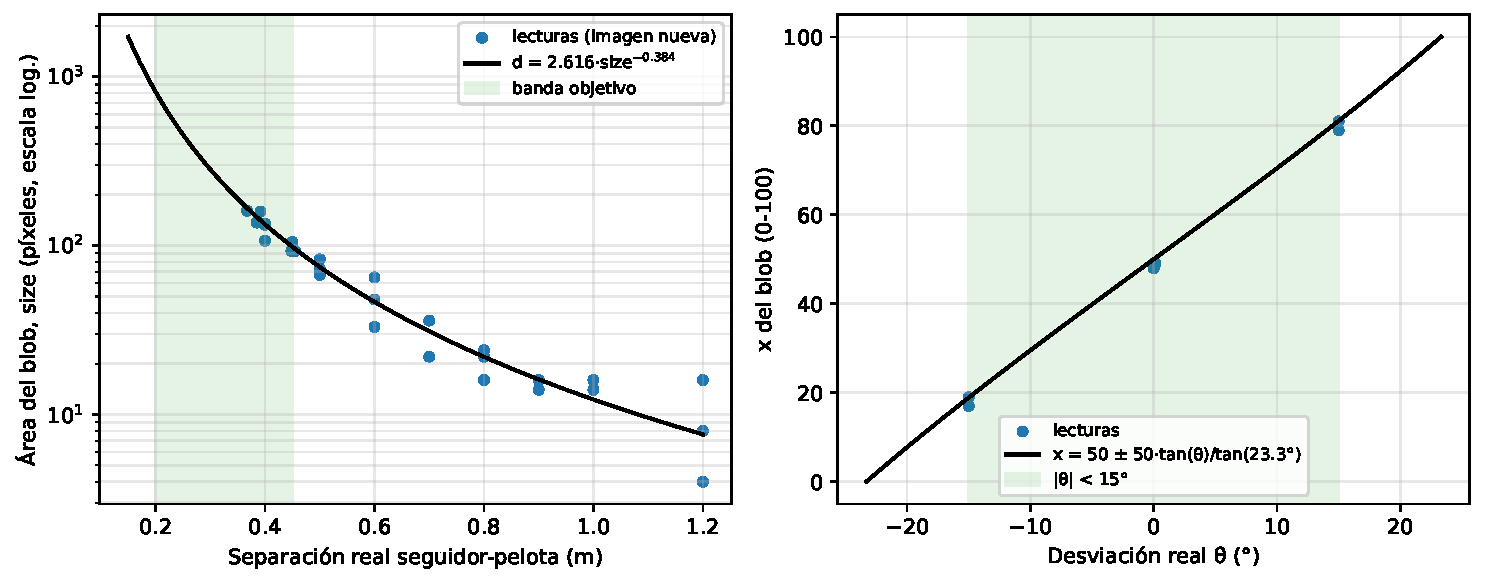
\includegraphics[width=\linewidth]{caracterizacion.pdf}
\caption{Caracterización del detector. Izquierda: área del blob frente a la separación y modelo
$d=2{,}616\cdot\text{size}^{-0{,}384}$. Derecha: $x$ del blob frente a la desviación, con un campo de visión de
46,6°.}
\label{fig:caract}
\end{figure}

\begin{figure}[h]
\centering
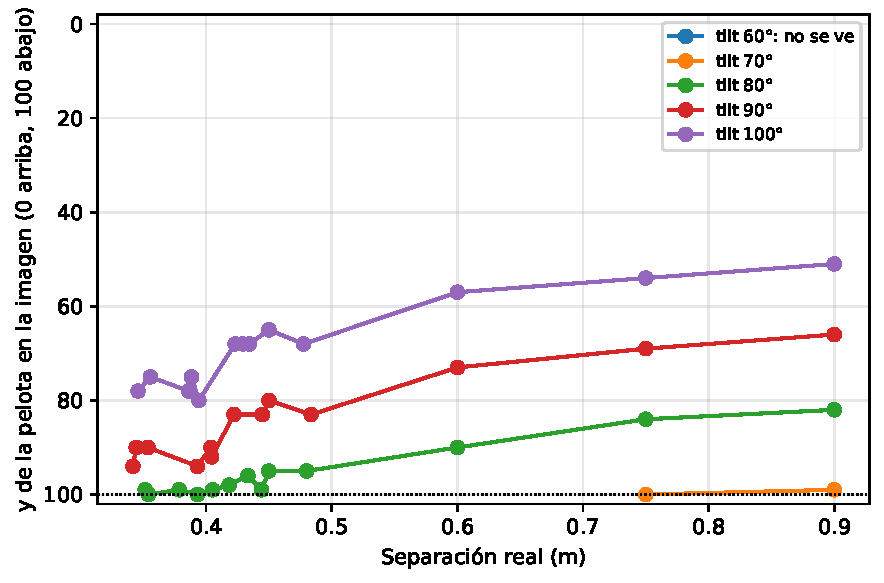
\includegraphics[width=0.55\linewidth]{barrido_tilt.pdf}
\caption{Altura de la pelota en la imagen según la inclinación de la cámara. Con 100° se ve en todo el rango
de interés.}
\label{fig:tilt}
\end{figure}

\begin{figure}[p]
\centering
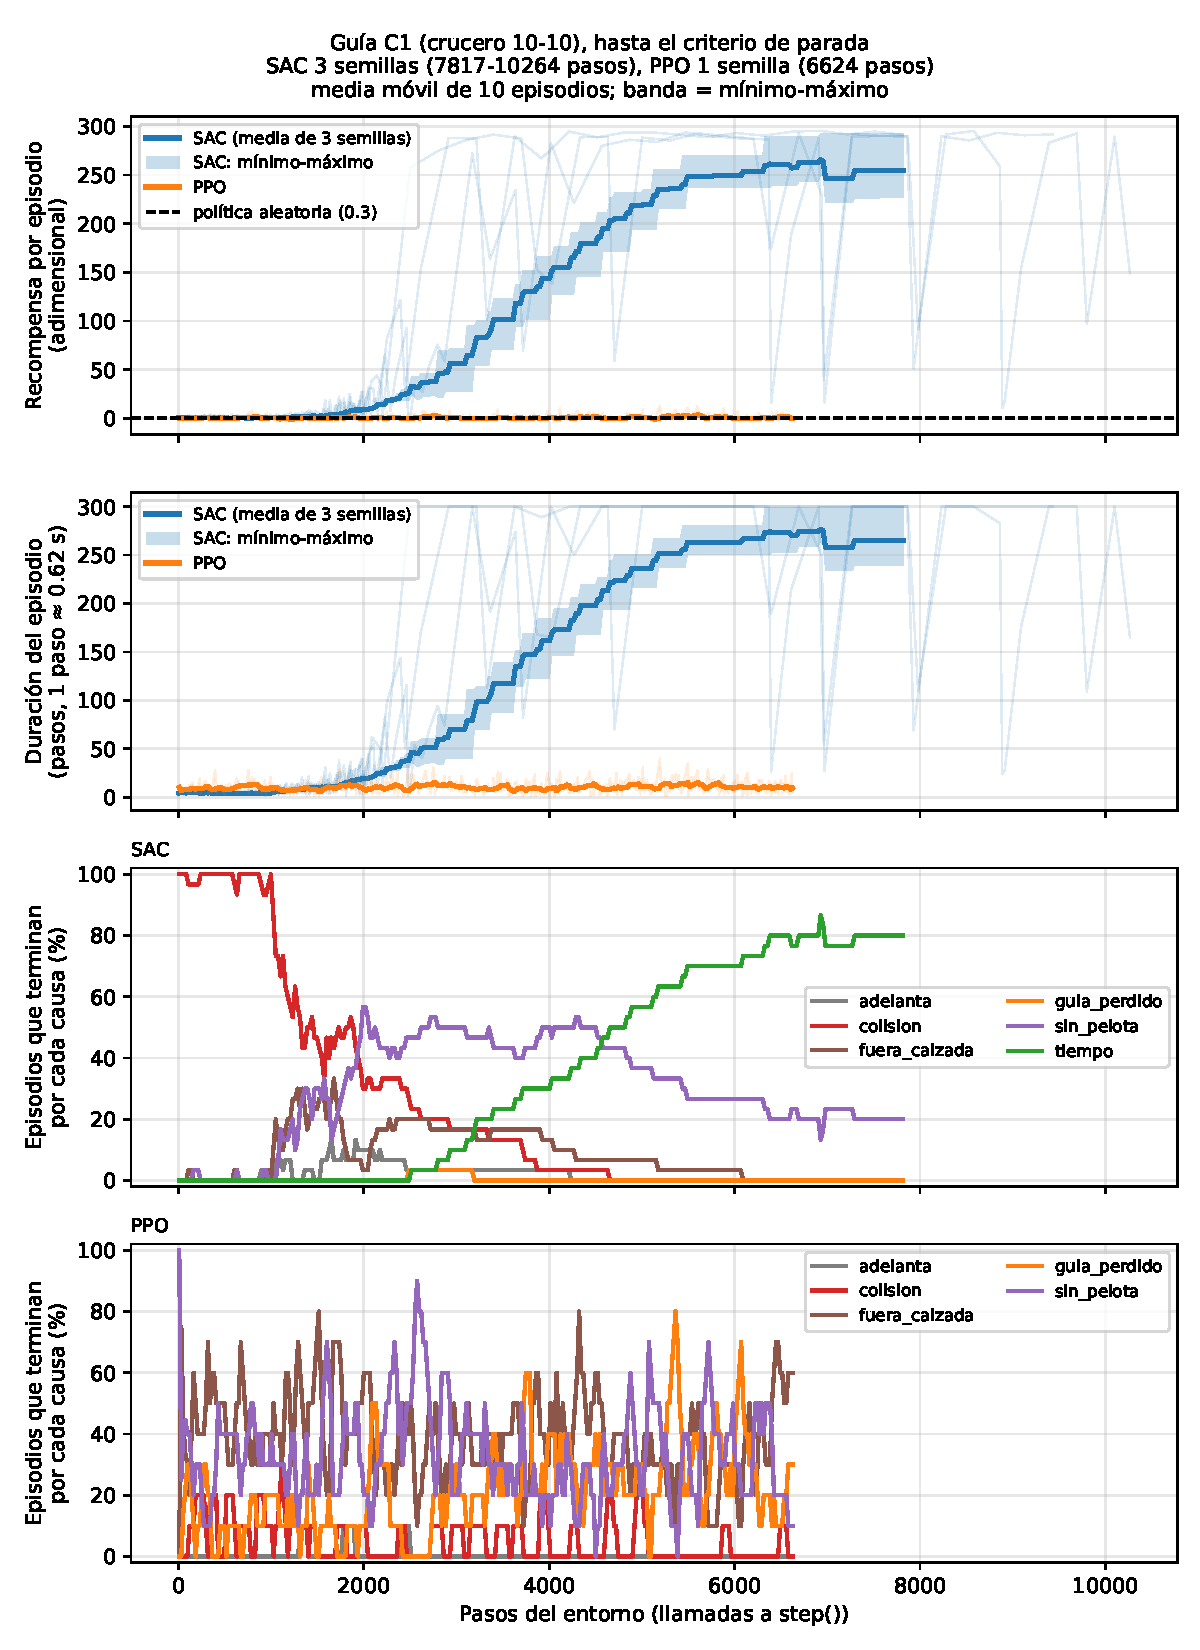
\includegraphics[height=0.85\textheight]{curvas_C1.pdf}
\caption{C1 (crucero 10--10): SAC con 3 semillas (media y banda mínimo--máximo; 7\,817--10\,264 pasos) y PPO con 1
semilla (6\,624 pasos). 1 paso $\approx$ 0,62~s.}
\label{fig:C1}
\end{figure}

\begin{figure}[p]
\centering
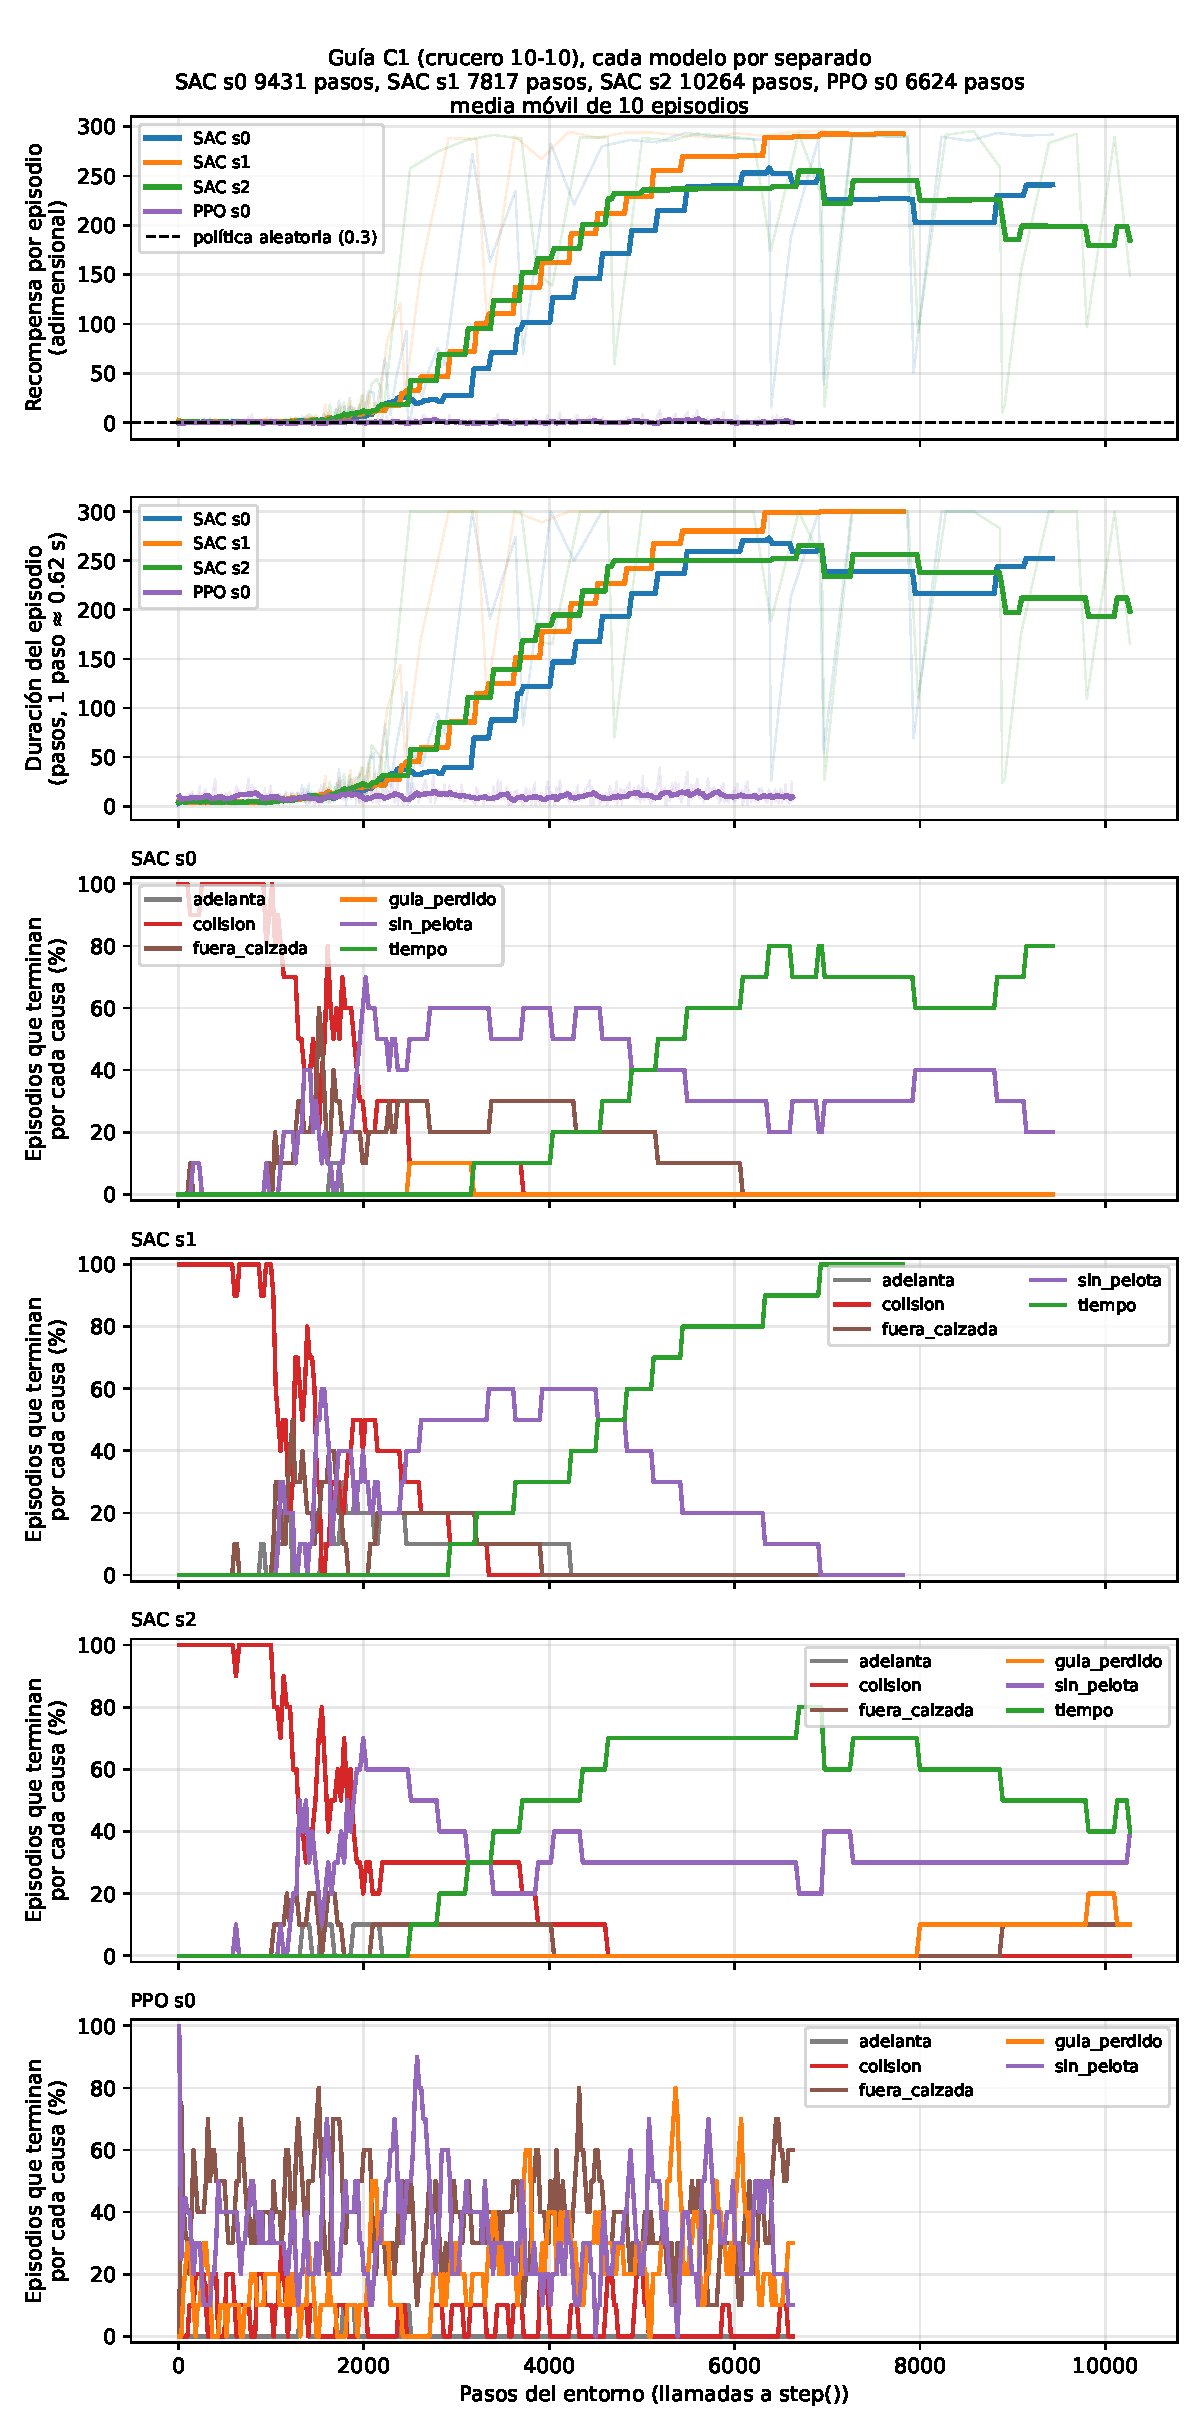
\includegraphics[height=0.85\textheight]{curvas_C1_modelos.pdf}
\caption{C1, cada modelo por separado.}
\label{fig:C1mod}
\end{figure}

\begin{figure}[p]
\centering
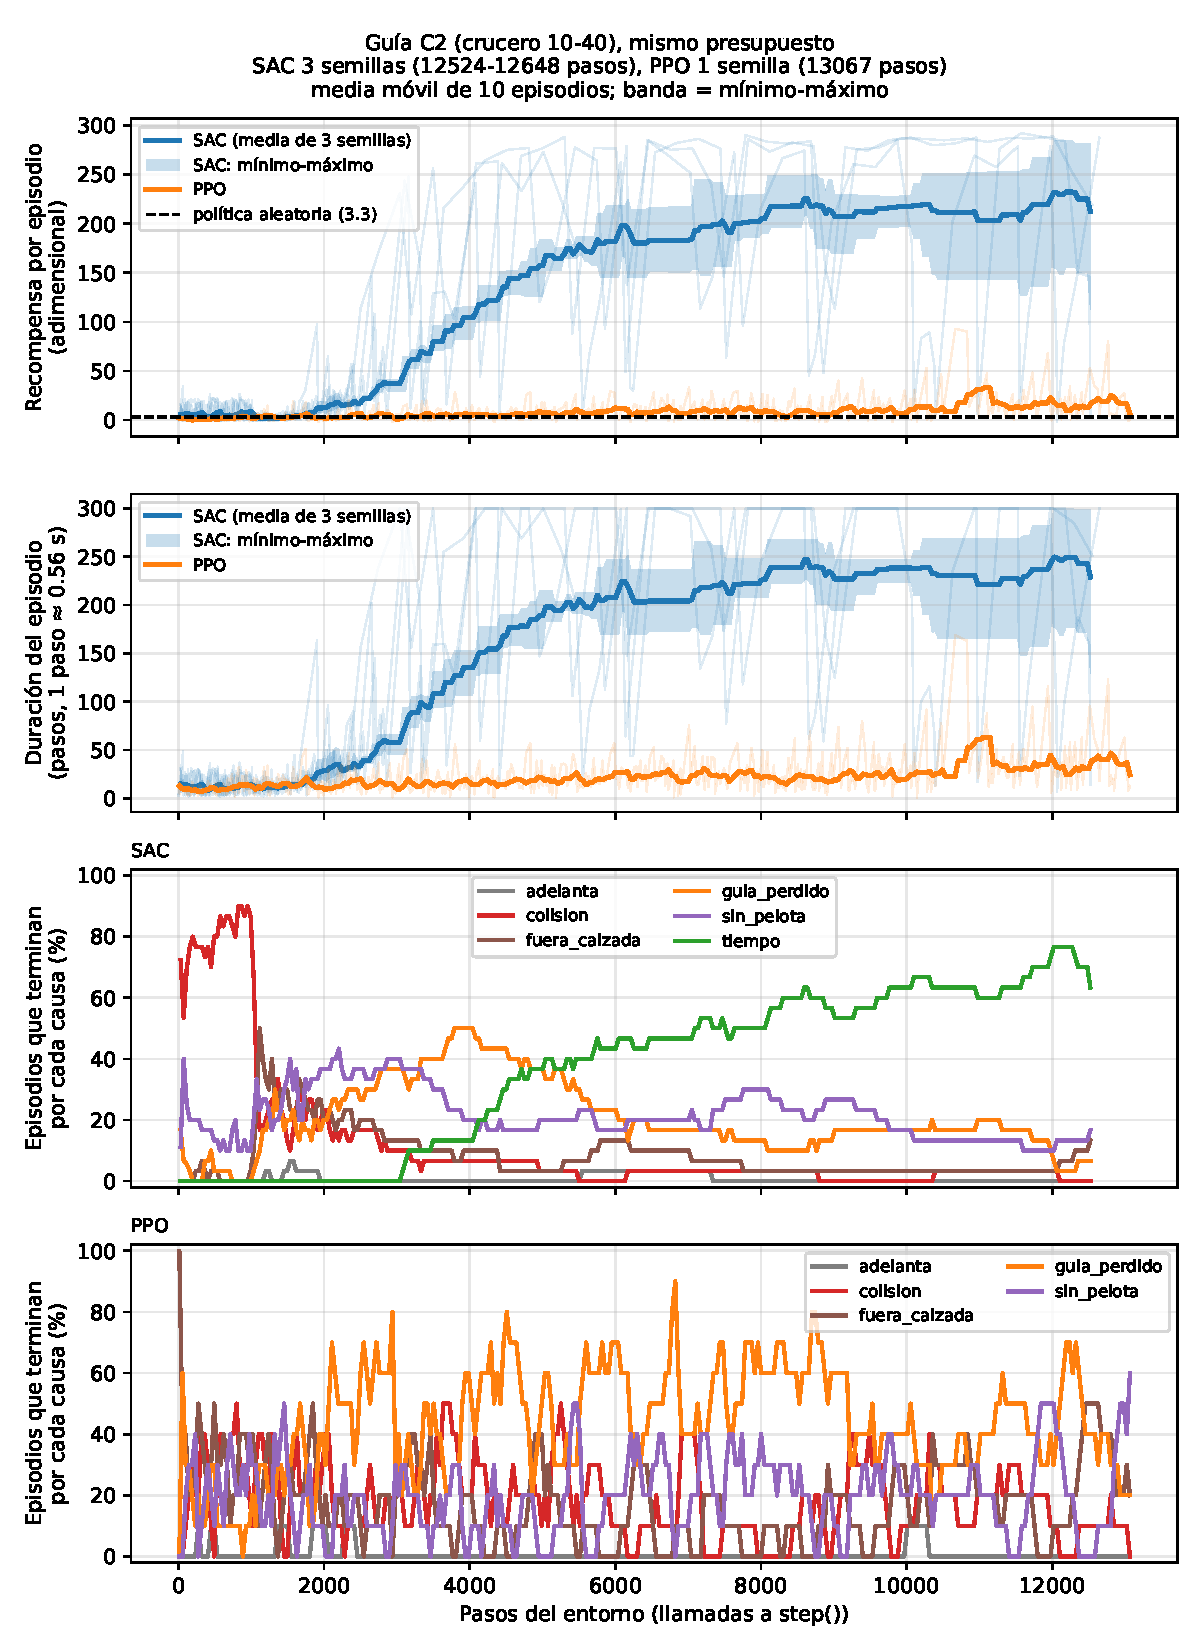
\includegraphics[height=0.85\textheight]{curvas_C2.pdf}
\caption{C2 (crucero 10--40), mismo presupuesto: SAC con 3 semillas (12\,524--12\,648 pasos) y PPO con 1 semilla
(13\,067 pasos). 1 paso $\approx$ 0,56~s.}
\label{fig:C2}
\end{figure}

\begin{figure}[p]
\centering
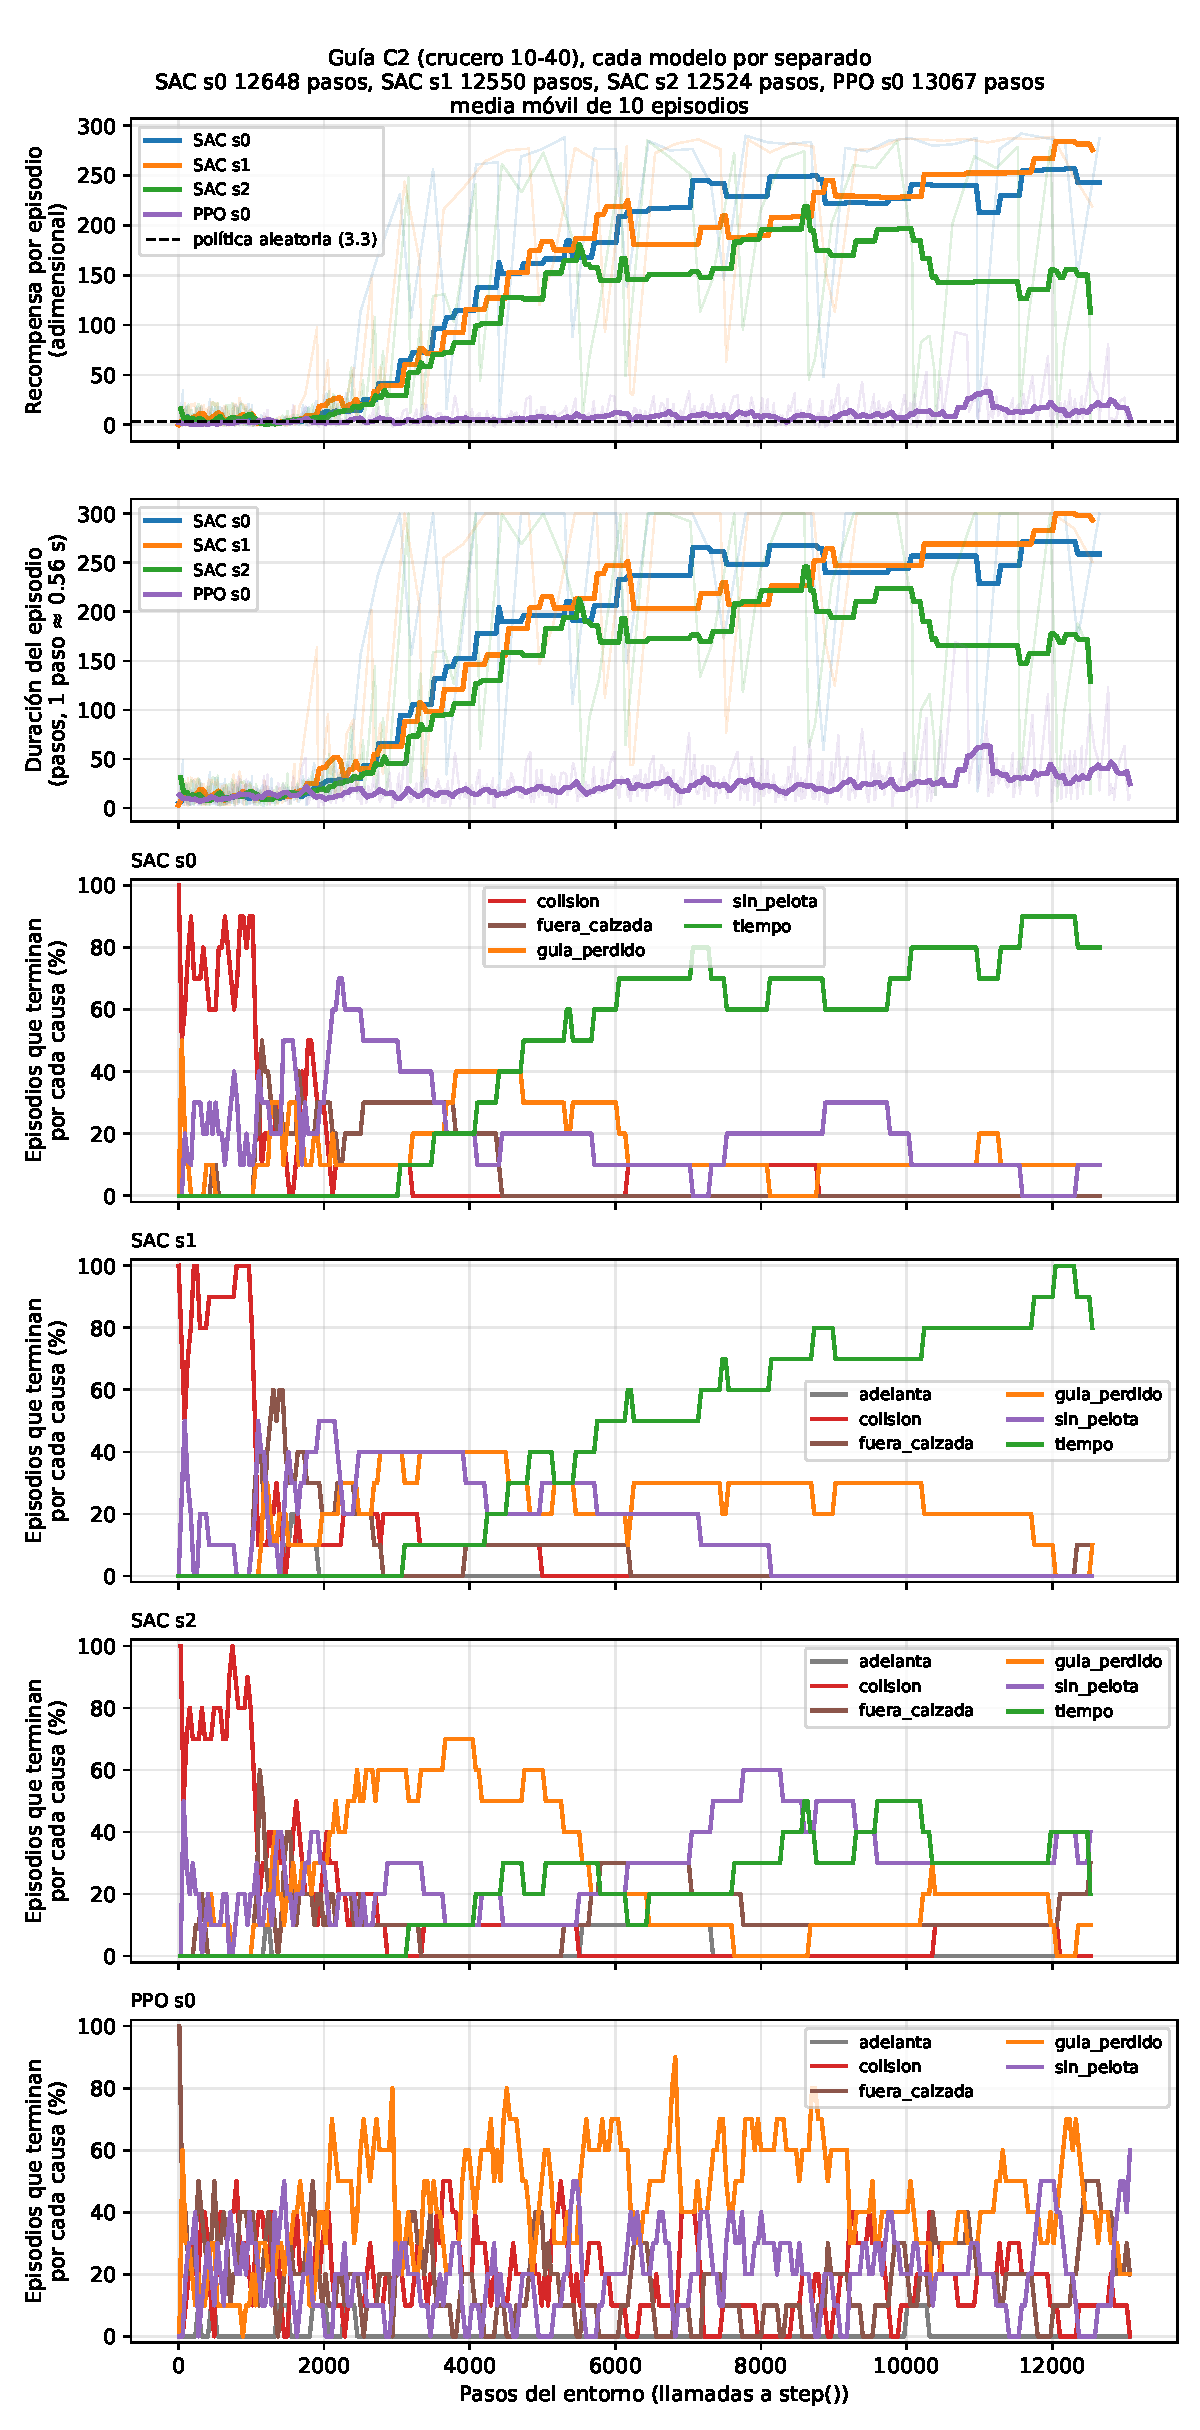
\includegraphics[height=0.85\textheight]{curvas_C2_modelos.pdf}
\caption{C2, cada modelo por separado, con el mismo presupuesto.}
\label{fig:C2mod}
\end{figure}

\begin{figure}[p]
\centering
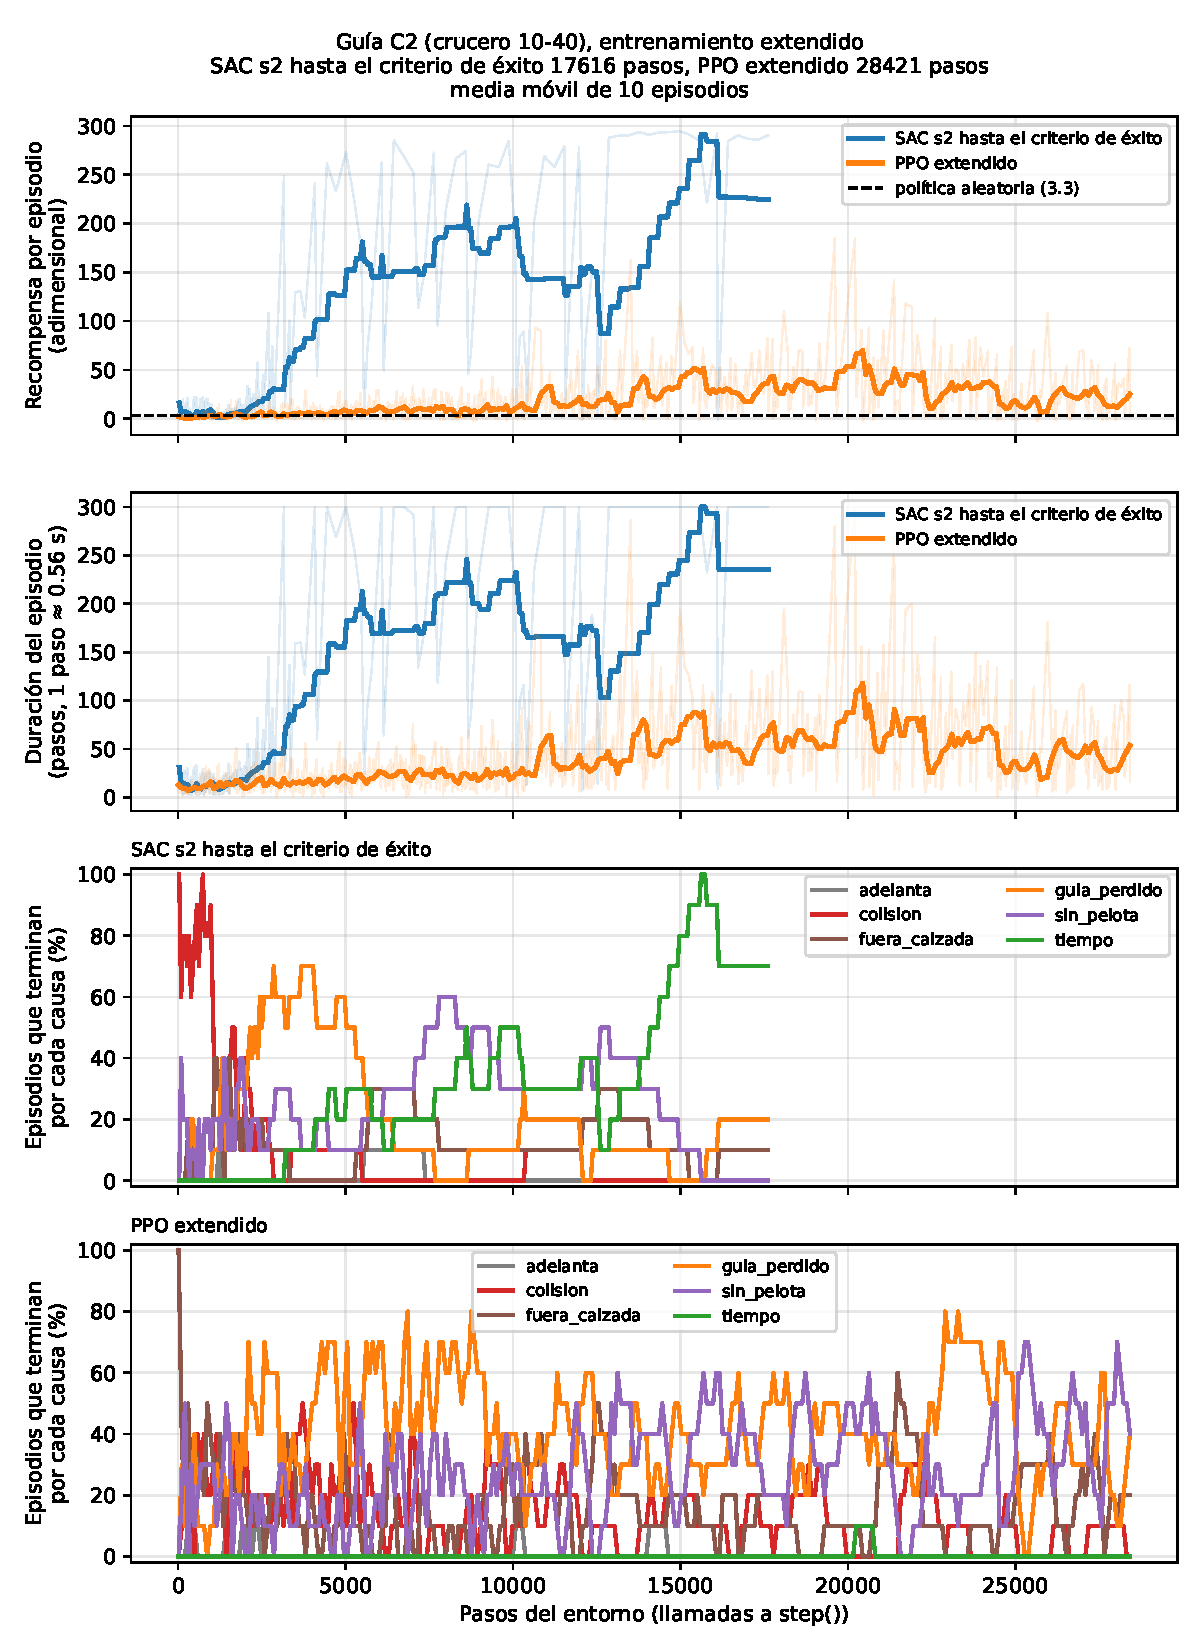
\includegraphics[height=0.85\textheight]{curvas_C2_ext.pdf}
\caption{C2, entrenamientos extendidos: SAC s2 hasta el criterio de éxito (17\,616 pasos) y PPO (28\,421 pasos).}
\label{fig:C2ext}
\end{figure}

\begin{figure}[p]
\centering
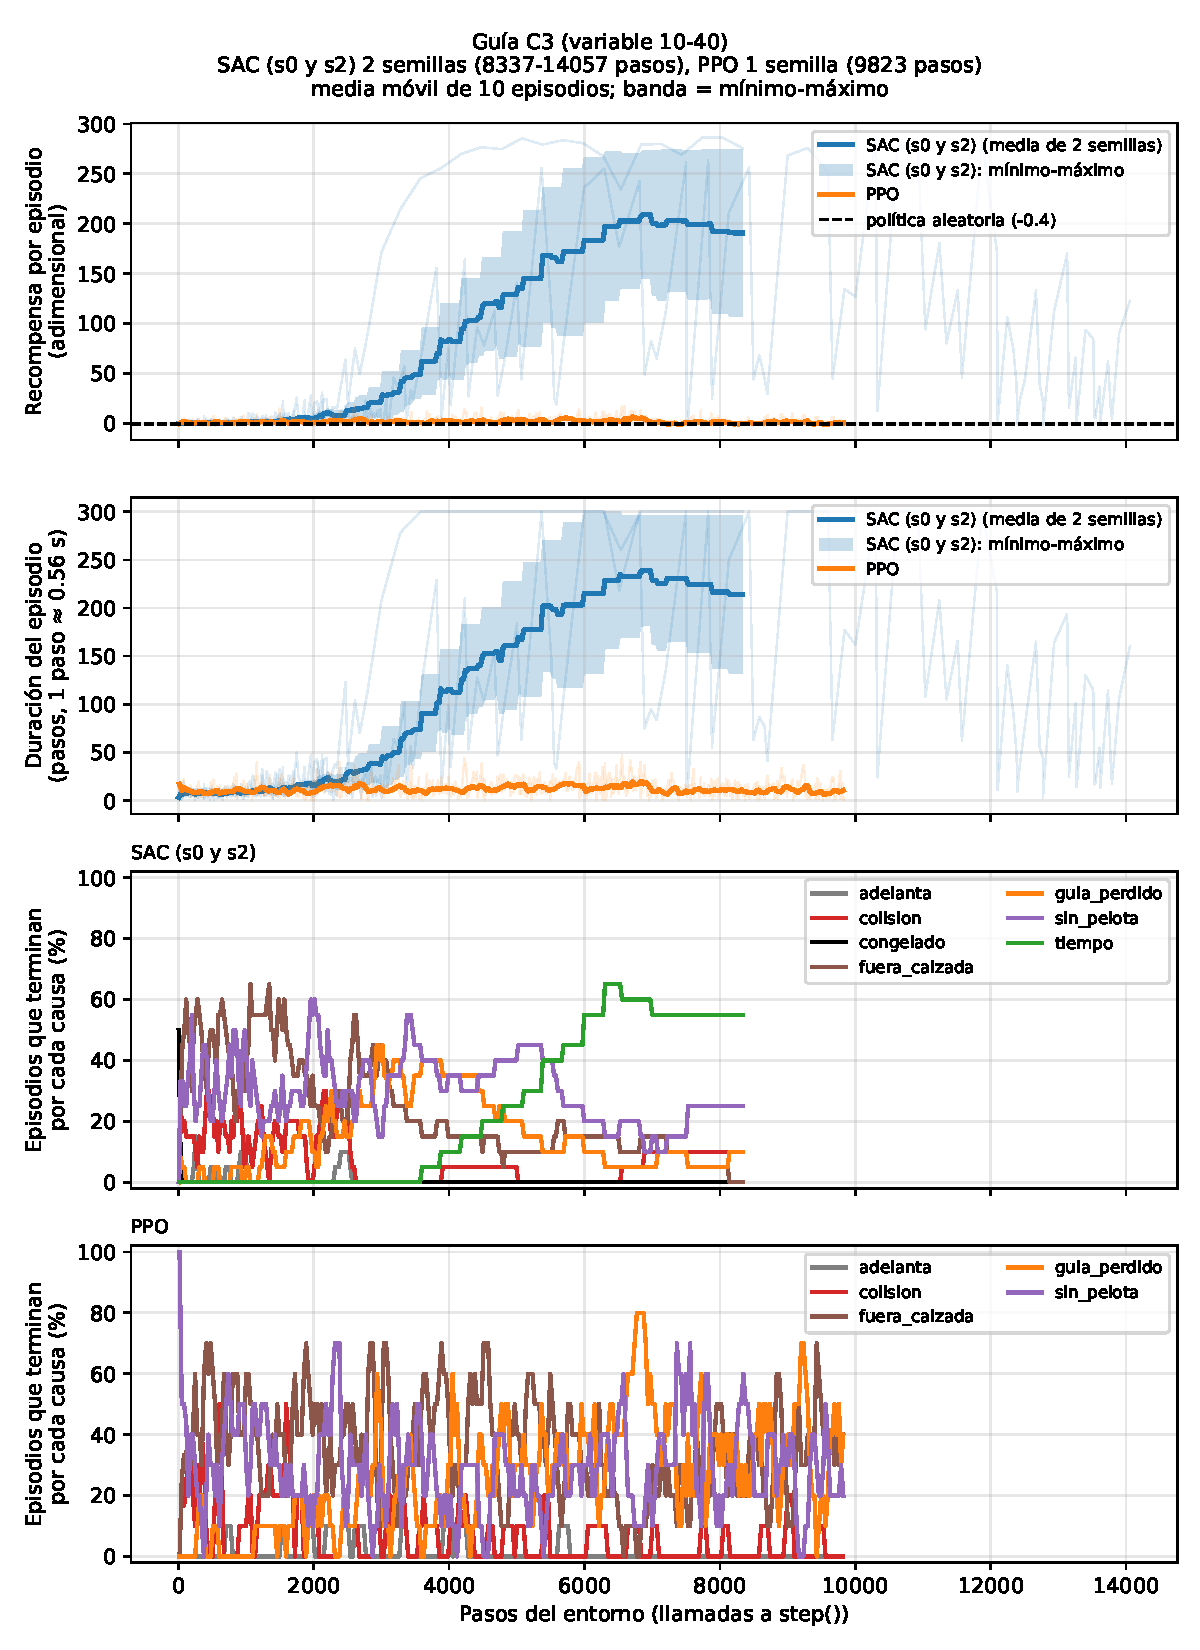
\includegraphics[height=0.85\textheight]{curvas_C3.pdf}
\caption{C3 (variable 10--40): SAC con 2 semillas (s0 y s2; 8\,337--14\,057 pasos) y PPO con 1 semilla (9\,823 pasos).
La semilla 1 se excluye por el fallo de percepción descrito en el apartado 4.3.}
\label{fig:C3}
\end{figure}

\begin{figure}[p]
\centering
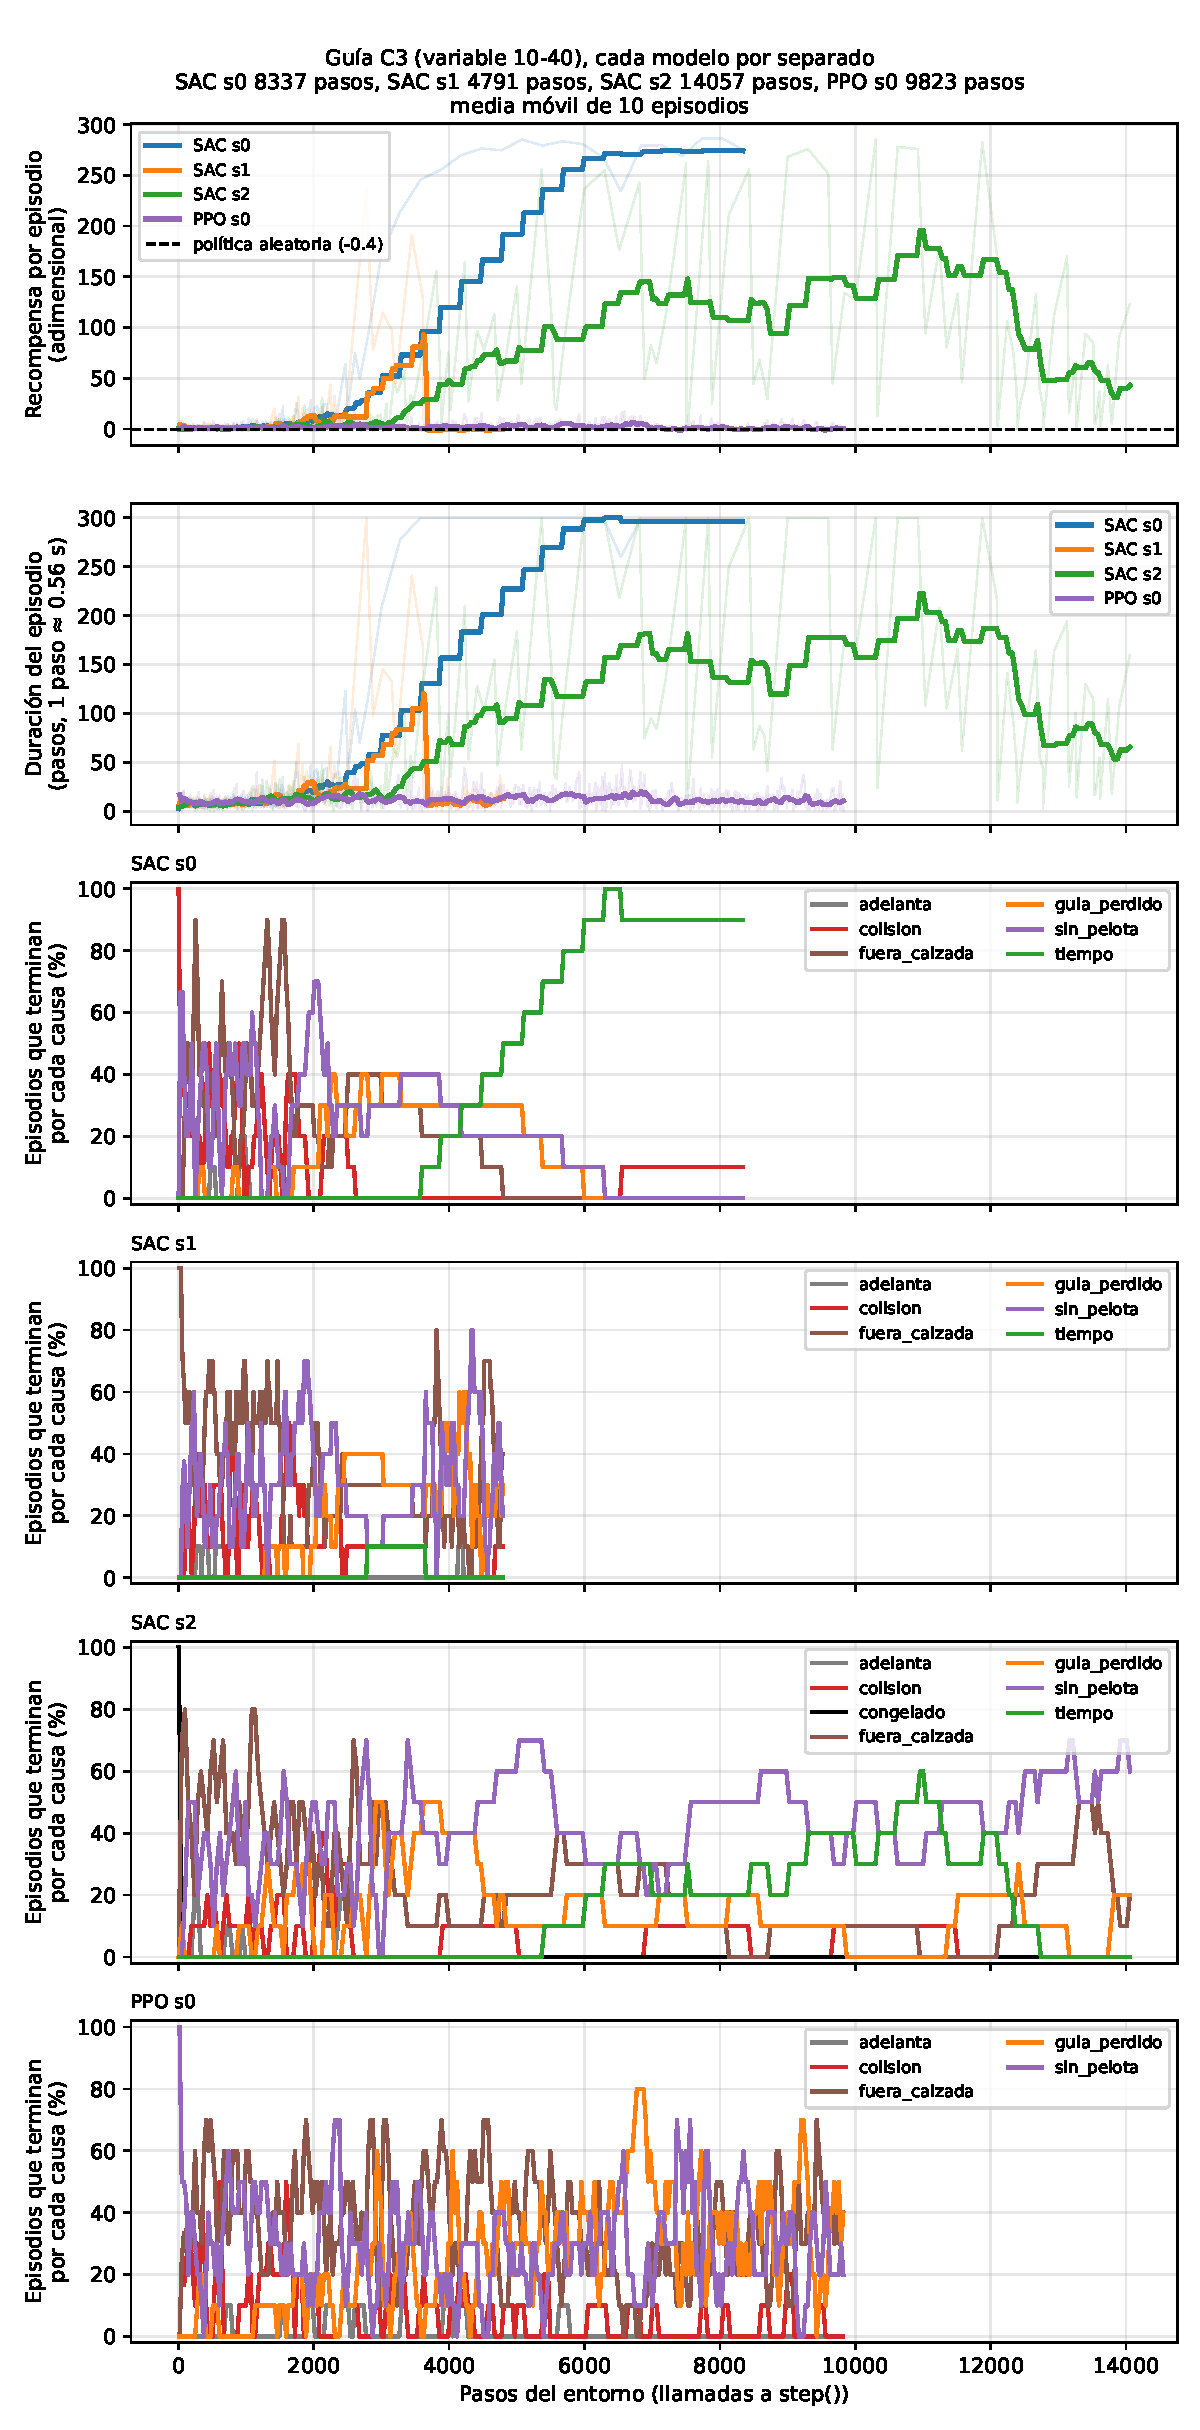
\includegraphics[height=0.85\textheight]{curvas_C3_modelos.pdf}
\caption{C3, cada modelo por separado. En SAC s1 se aprecia la caída brusca hacia el paso 3\,615 causada por el
fallo de percepción.}
\label{fig:C3mod}
\end{figure}

\end{document}
